\section{Implantación}
\subsection{Código fuente completo (parcial)}
\begin{figure}[H]
	\centering
	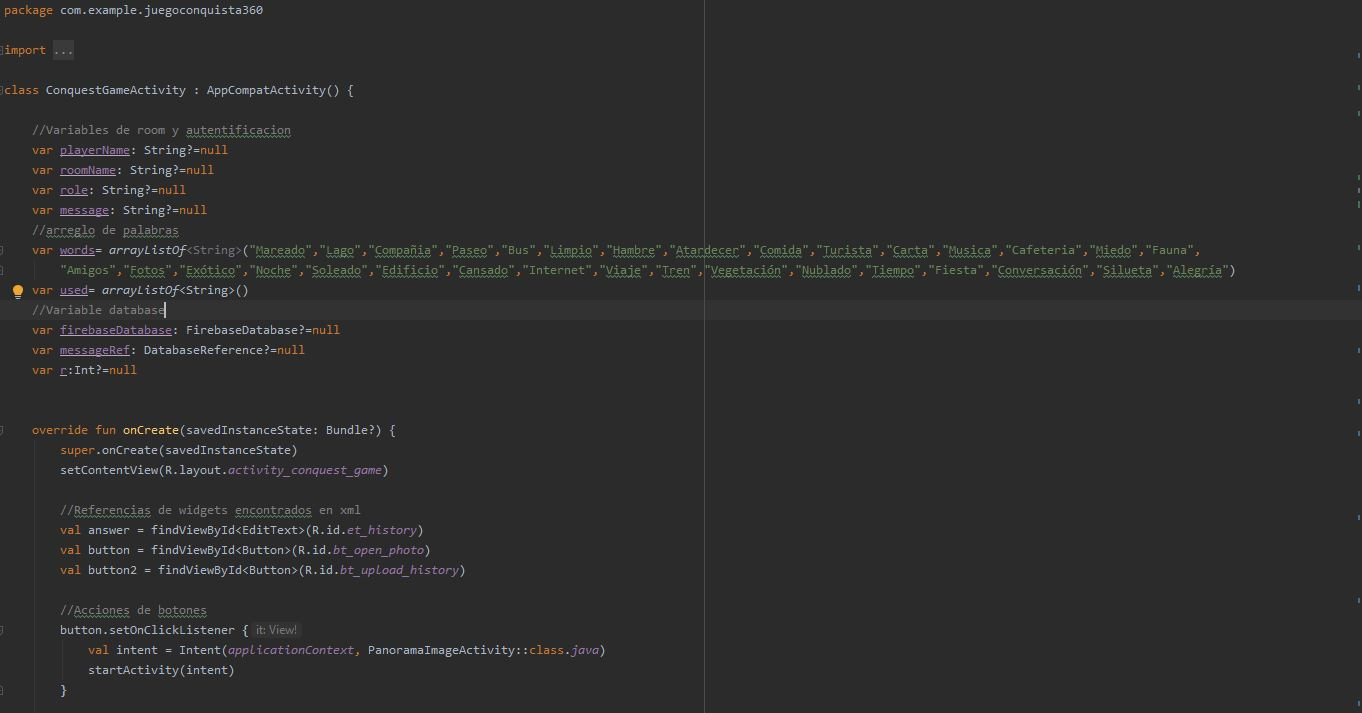
\includegraphics[width=16cm, height=9cm]{imgs/SourceCode1.jpg}
	\caption{Codigo Clase ConquestGameActivity parte 1}
\end{figure}
\begin{figure}[H]
	\centering
	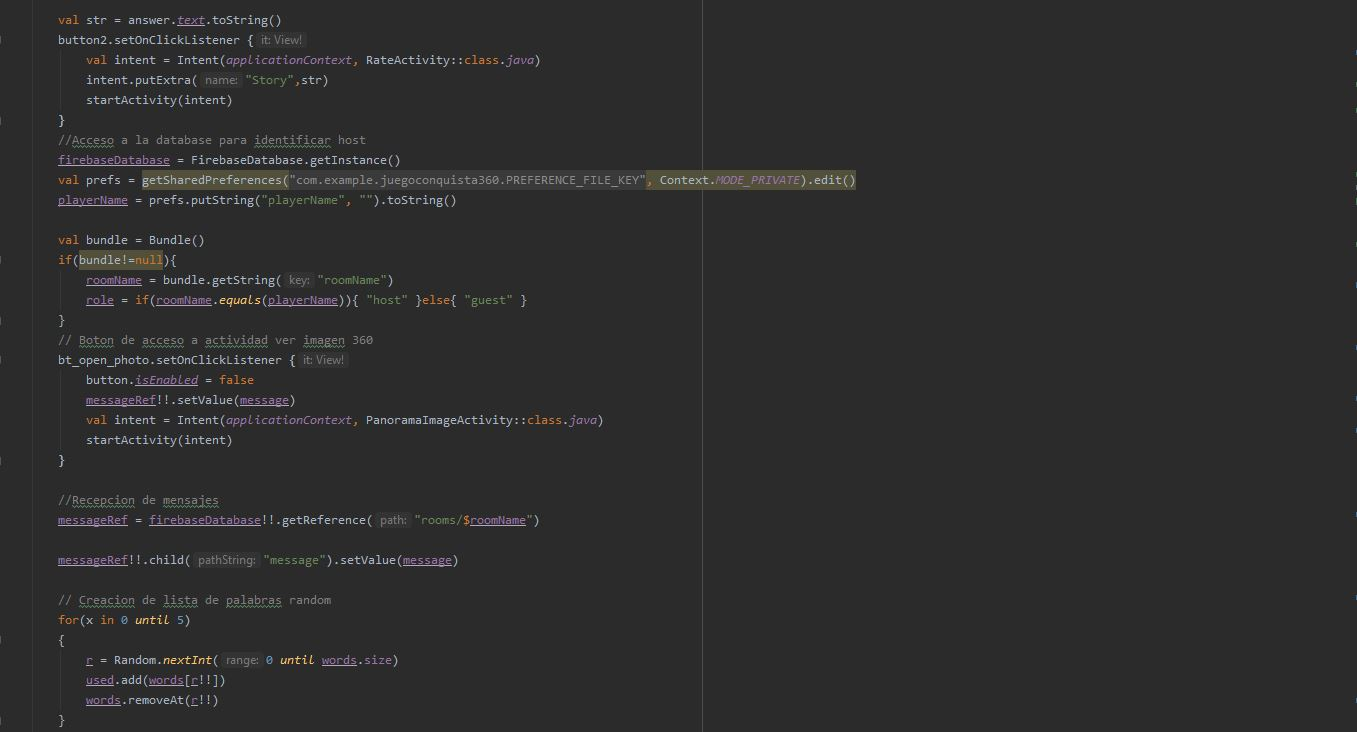
\includegraphics[width=16cm, height=9cm]{imgs/SourceCode2.jpg}
	\caption{Codigo Clase ConquestGameActivity parte 2}
\end{figure}
\begin{figure}[H]
	\centering
	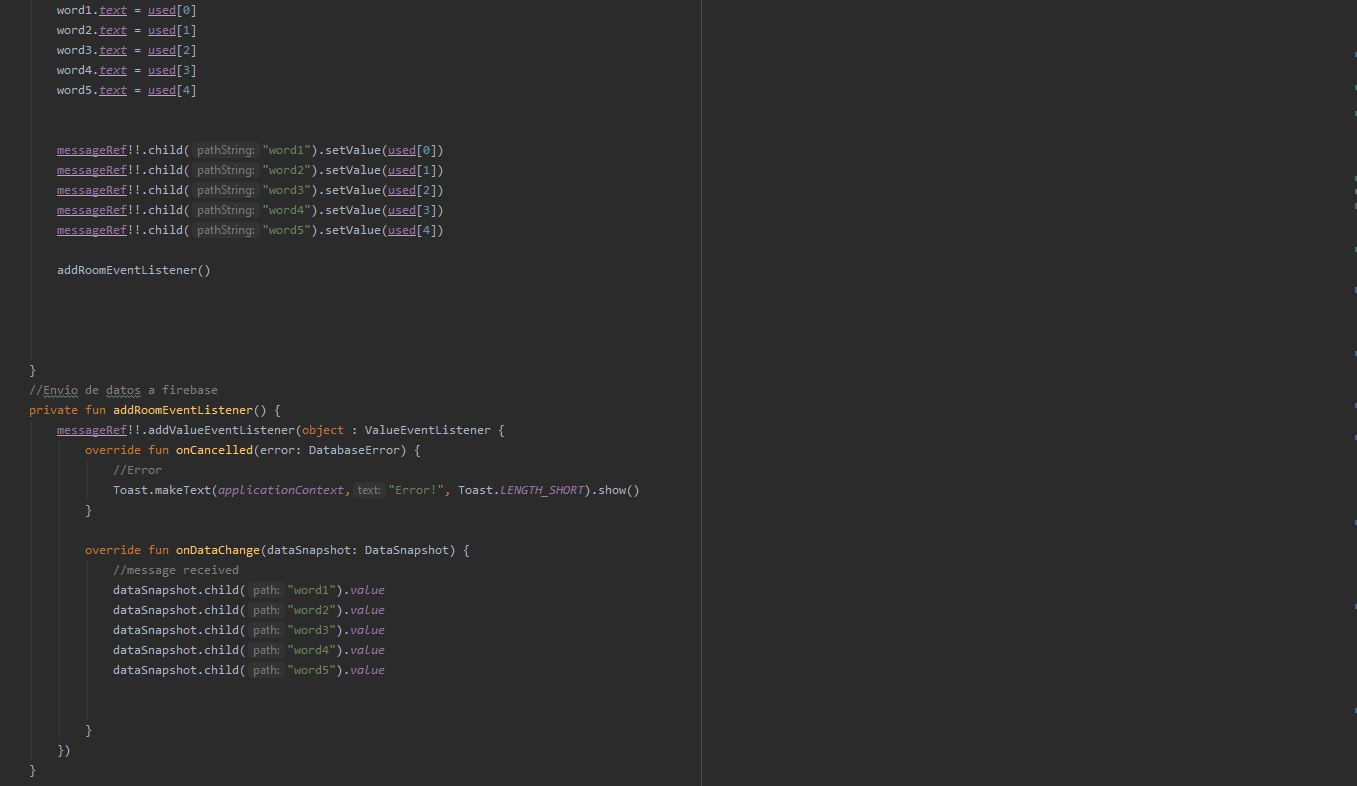
\includegraphics[width=16cm, height=9cm]{imgs/SourceCode3.jpg}
	\caption{Codigo Clase ConquestGameActivity parte 3}
\end{figure}
\subsection{Dependencias}
Firebase: Es requerido para poder gestionar el inicio de sesión junto con la información requerida
que necesite ser guardada, ya que posee una base de datos en tiempo real y gestionará cuando un jugador suba una historia, cuando los jugadores evaluen dicha historia, etc.

Giroscopio: Es necesario para que el jugador pueda ver girar y ver la imagen en 360°


